% $Header: /cvsroot/latex-beamer/latex-beamer/examples/beamerexample1.tex,v 1.47 2004/11/04 15:43:51 tantau Exp $

%%% FOR PRESENTATION
%\documentclass{beamer}
%%%\documentclass[notes]{beamer}
%%% FOR HANDOUT
%\documentclass[notes,handout]{beamer}
%%%%%%\documentclass[notes,handout]{beamer}

%\documentclass{article}
%\usepackage[envcountsect]{beamerarticle}

% Do NOT take this file as a template for your own talks. Use a file
% in the directory solutions instead. They are much better suited.

% Try the class options [notes], [notes=only], [trans], [handout],
% [red], [compress], [draft] and see what happens!

% Copyright 2003 by Till Tantau <tantau@users.sourceforge.net>.
%
% This program can be redistributed and/or modified under the terms
% of the LaTeX Project Public License Distributed from CTAN
% archives in directory macros/latex/base/lppl.txt.


%\mode<presentation>
%{
  %\usetheme{Malmoe} %Luebeck
  %\usefonttheme[onlysmall]{structurebold}
  %\setbeamertemplate{background canvas}[vertical shading][bottom=gray!5,top=gray!5]
  %\usecolortheme{dolphin}
%}
%\setbeamercovered{transparent}
%\setbeamercolor{math text}{fg=green!50!black}
%\setbeamercolor{normal text in math text}{parent=math text}

%\usepackage{pgf,pgfarrows,pgfnodes,pgfautomata,pgfheaps,pgfshade}
%\usepackage{amsmath,amssymb}
%\usepackage[latin1]{inputenc}
%\usepackage{wasysym}
%\usepackage{colortbl}
%\usepackage[english]{babel}
%\usepackage{color}
%\usepackage{listings}         % Auflistung von Ausschnitten von Programm-Code
%\usepackage{bibgerm}
%\bibliographystyle{acm}

%\usepackage{xcolor}     %for listings
%\usepackage{fancybox} 

%\usepackage{pgfpages}
%\pgfpagelayout{2 on 1}[a4paper,border shrink=5mm,landscape]

%\usepackage{lmodern}
%\usepackage[T1]{fontenc} 

%\usepackage{times}

%%%%%%%%%%%%%%%%%%%%%%%%%%%%%%%%%%%
%%%       MODIFY  FOOTLINE      %%%
%%%%%%%%%%%%%%%%%%%%%%%%%%%%%%%%%%%
%\defbeamertemplate*{footline}{infolines theme}
%{
%  \leavevmode%
%  \hbox{%
%  \begin{beamercolorbox}[wd=.32\paperwidth,ht=2.25ex,dp=1ex,center]{author in head/foot}%
%    \usebeamerfont{author in head/foot}\insertshortauthor
%  \end{beamercolorbox}%
%  \begin{beamercolorbox}[wd=.58\paperwidth,ht=2.25ex,dp=1ex,center]{title in head/foot}%
%    \usebeamerfont{title in head/foot}\insertshorttitle
%  \end{beamercolorbox}%
%  \begin{beamercolorbox}[wd=.1\paperwidth,ht=2.25ex,dp=1ex,right]{date in head/foot}%
%    %\usebeamerfont{date in head/foot}\insertshortdate{}\hspace*{2em}
%    \insertframenumber{} / \inserttotalframenumber\hspace*{2ex} 
%  \end{beamercolorbox}}%
%  \vskip0pt%
%}
%%%%%%%%%%%%%%%%%%%%%%%%%%%%%%%%%%%


%\title[Model Execution in Eclipse]{Model Execution in Eclipse}
%\subtitle[KIELER Execution Manager]{KIELER Execution Manager}
%\author[Eclipse Summit 2009]{%
%  Christian~Motika}
%\institute[\myshortinstitute]{
%  Real-Time Systems and Embedded Systems Group\\
%  Department of Computer Science\\
  % Faculty of Engineering\\
%  Christian-Albrechts-Universit\"at zu Kiel, Germany
%}
%\date[Eclipse Summit 2009]{
%\begin{tabular}[h]{l l}
%   \parbox{0.30\textwidth}{
%   			{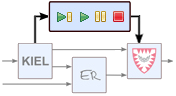
\includegraphics[scale=0.50]{./images/kiem-logo.png}}
%   }
%   \parbox{0.90\textwidth}{   
%				Eclipse Summit, 08/27/2009
%   }
%\end{tabular}
%}

%\subject{Model Execution in Eclipse}

%%% some new commands %%%
\newcommand{\BRED}[1]{\textbf{\textcolor[rgb]{0.50,0.00,0.00}{#1}}}
\newcommand{\BGREEN}[1]{\textbf{\textcolor[rgb]{0.00,0.50,0.00}{#1}}}
\newcommand{\RED}[1]{\textcolor[rgb]{0.80,0.00,0.00}{#1}}
\newcommand{\GREEN}[1]{\textcolor[rgb]{0.00,0.50,0.00}{#1}}
\newcommand{\GRAY}[1]{\textcolor[rgb]{0.60,0.60,0.60}{#1}}
\newcommand{\BLUE}[1]{\textcolor[rgb]{0.192,0.204,0.709}{#1}}

%% font Courier for the (programming) code
%\usepackage{courier}
%% new command \code{text}
\newcommand{\code}[1]{{\fontfamily{pcr}\selectfont #1}}
%% new command for quotations
\newcommand{\myquote}[1]{\glqq #1\grqq}

%% new command for code listings
%% \usepackage{listings} (s.a.)
\lstloadlanguages{XML}
\lstloadlanguages{C++}
\lstloadlanguages{Java}
\newcommand{\listingjava}{
  \lstset{
  basicstyle=\tiny\tt, 
	numbers=left,
	frame=shadowbox,rulesepcolor=\color{lightgray},
	morecomment=[l]{//},
	tabsize=3,
	language=Java,
	keywordstyle=\bfseries\color[rgb]{0.482,0,0.323},
	stringstyle=\color{blue},
	commentstyle=\color[rgb]{0.224,0.49,0.353},
	numberstyle=\tiny,
	showstringspaces=false,
	backgroundcolor=\color[rgb]{1,1,0.74},
	emph={xxx},
	emphstyle=\color{blue}
}}

\newcommand{\listingxml}{
  \lstset{
  basicstyle=\tiny\tt, 
	numbers=left,
	frame=shadowbox,rulesepcolor=\color{lightgray},
	morecomment=[l]{//},
	tabsize=3,
	language=C,
	keywordstyle=,
	numberstyle=\tiny,
	showstringspaces=false,
	backgroundcolor=\color[rgb]{0.95,0.95,0.95}  
}}


 \newcommand\BackgroundPicture[1]{%
    \setbeamertemplate{background}{%
    \parbox[c][\paperheight]{\paperwidth}{%
        \vfill \hfill
 \includegraphics[width=0.8\paperwidth,height=0.8\paperheight]{#1}
         \hfill \vfill
      }}}


\newcommand{\showlisting}[2]{{
 \tiny
 \lstinputlisting[language=#2]{#1} 
 \normalsize
 }
}

%\setbeamerfont*{normaltext}{size=\scriptsize, series=\bfseries}

%\begin{document}
%standard font for slides
\small

%set the background image
\BackgroundPicture{images/kiembackground1.png}

%\part<presentation>{Main Talk}
%\frame{\titlepage}
%\note{}

\section*{Introduction}


\subsection<presentation>[Motivation]{Motivation}
%%%%%%%%%%%%%%%%%%%% Folie 1 %%%%%%%%%%%%%%%%%%%%%%%%

\begin{frame}
  \frametitle{Motivation}
  \begin{block}{}
    \begin{itemize}
	      \item \RED{EMF and GMF} are great frameworks for modeling in \RED{Eclipse}
	      \pause
	      \item Model implementations, model and diagram editors, ...
	      \pause
	      \item Modeling:
					\begin{enumerate}
							\item Structural models 
							\begin{itemize}
									\item E.g., class diagrams, component diagrams, ...
							\end{itemize}
							\pause
							\item Behavioral models
							\begin{itemize}
									\item E.g., flow charts, state machines, data flow models, ...
							\end{itemize}
					\end{enumerate}
    \end{itemize}
  \end{block}
\end{frame}
%\note{} 



%%%%%%%%%%%%%%%%%%%% Folie 2 %%%%%%%%%%%%%%%%%%%%%%%%
\begin{frame}
  \frametitle{Motivation (cont'd)}
  \begin{block}{}
\begin{center}
   \fbox{\parbox{100mm}{
   \normalsize{
\emph{System models} are virtual as opposed to physical systems
}}}
\end{center}
\small
\pause
    \begin{itemize}
	      \item System models
						\begin{itemize}
							\item Generate code or documentation
							\item System analysis and verification
							\item Simulation runs
							\item ...
						\end{itemize}
	      \pause
	      \item \textbf{Idea:} Flexible definition of semantics and swapping out of simulation computation 
	      \pause	
	      \item \textbf{Solution proposed:} \RED{KIELER Execution Manager}
    \end{itemize}
  \end{block}
\end{frame}
%\note{} 



\subsection<presentation>[Overview]{Overview}
%%%%%%%%%%%%%%%%%%%% Folie 3 %%%%%%%%%%%%%%%%%%%%%%%%
\begin{frame}
  \frametitle{Overview}
    \begin{itemize}
	      \item KIELER Execution Manager
	      \pause
	      \item Use case: Ptolemy 
        \begin{itemize}
       	       \item M2M transformation
       	       \item Simulation engine
	             \pause
        \end{itemize}
	      \item Use case: Model Railway
        \begin{itemize}
	            \item Installation
	            \item Railway Controller DSL
	            \item SimpleRailCtrl editor \emph{(DEMO)}
        \end{itemize}
        \pause
	      \item Summary
    \end{itemize}
\end{frame}
%\note{} 

\section[KIELER Execution Manager]{KIELER Execution Manager}

\subsection[DataComponents]{DataComponents}
%%%%%%%%%%%%%%%%%%%% Folie 4 %%%%%%%%%%%%%%%%%%%%%%%%
\begin{frame}
  \frametitle{KIEM Components}
			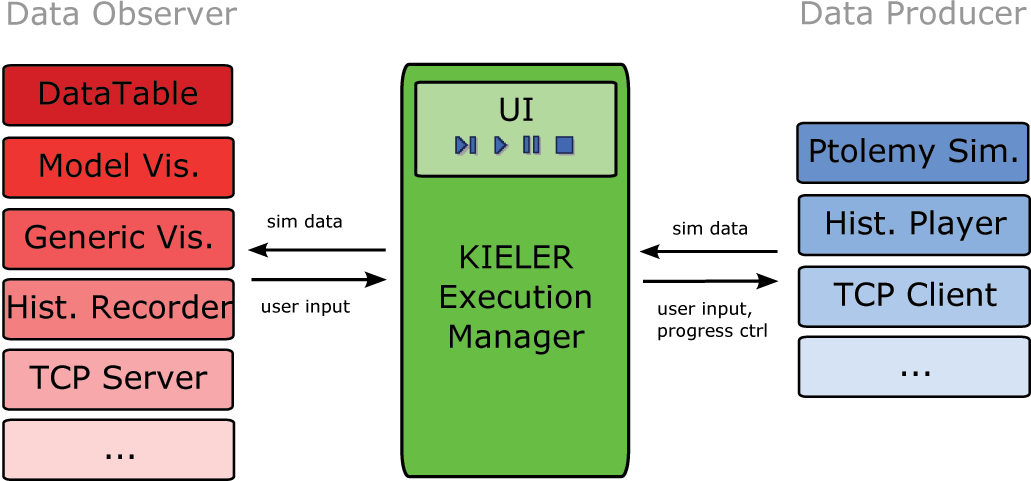
\includegraphics[scale=0.30]{images/kiem.png}
  \end{frame}
%\note{} 


\subsection[GUI And Threads]{GUI And Threads}
%%%%%%%%%%%%%%%%%%%% Folie 5 %%%%%%%%%%%%%%%%%%%%%%%%
\begin{frame}
  \frametitle{KIEM GUI and Threads}
  			\begin{tabular}[h]{l r}
			   \parbox{0.56\textwidth}{
			\only<1>{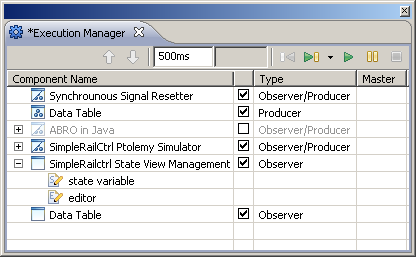
\includegraphics[scale=0.41]{images/kiem-view.png}}
%			\only<2>{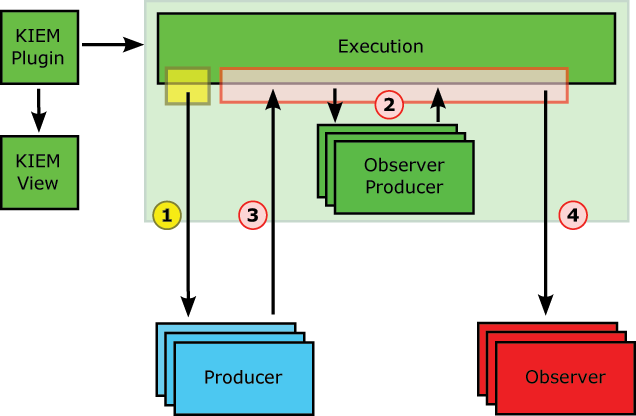
\includegraphics[scale=0.27]{images/kiem-threads.png}}
%			\only<3->{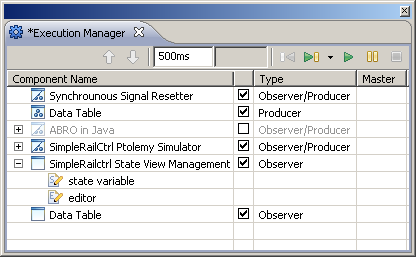
\includegraphics[scale=0.41]{images/kiem-view.png}}
			}
   			\parbox{0.44\textwidth}{   
\begin{itemize}
	\item DataObserver vs. DataProducer
	\pause
	\item Scheduling $\&$ DataPool
	\pause
	\item Properties
	\pause
	\item Execution Buttons
	\pause
	\item Master
\end{itemize}
}
		\end{tabular}	

  \end{frame}
%\note{} 


\subsection[Interface]{Interface}
%%%%%%%%%%%%%%%%%%%% Folie 6 %%%%%%%%%%%%%%%%%%%%%%%%
\begin{frame}
  \frametitle{Simple Interface}
  \begin{center} 
				\listingjava \showlisting{code/Interface.java}{Java} 
  \end{center}
\end{frame}
%\note{} 

\begin{frame}
%%%%%%%%%%%%%%%%%%%% Folie 7 %%%%%%%%%%%%%%%%%%%%%%%%
  \frametitle{Flexible Extensions}
  \begin{center} 
				\listingjava \showlisting{code/Extensions.java}{Java} 
  \end{center}
\end{frame}
%\note{} 


\section[Use Case: Ptolemy]{Use Case: Ptolemy}
%%%%%%%%%%%%%%%%%%%% Folie 8 %%%%%%%%%%%%%%%%%%%%%%%%
\begin{frame}
  \frametitle{Overview}
    \begin{itemize}
	      \item \GRAY{KIELER Execution Manager}
	      \item Use case: Ptolemy 
        \begin{itemize}
       	       \item M2M transformation
       	       \item Simulation engine
        \end{itemize}
	      \item \GRAY{Use case: Model Railway}
        \begin{itemize}
	            \item \GRAY{Installation}
	            \item \GRAY{Railway Controller DSL}
	            \item \GRAY{SimpleRailCtrl editor \emph{(DEMO)}}
        \end{itemize}
	      \item \GRAY{Summary}
    \end{itemize}
\end{frame}
%\note{} 

%%%%%%%%%%%%%%%%%%%% Folie 9 %%%%%%%%%%%%%%%%%%%%%%%%
\begin{frame}
  \frametitle{What is Ptolemy?}
  
\begin{center}
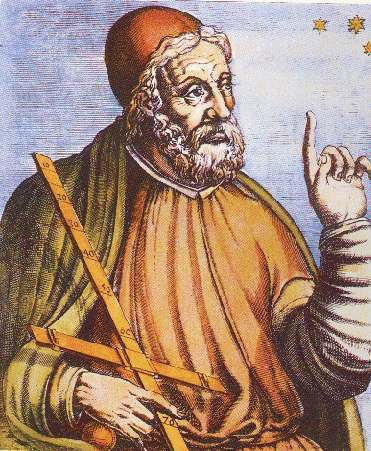
\includegraphics[scale=0.20]{images/clausptolemaeus.jpg}
\end{center}
  
\begin{itemize}
	\item \myquote{The Ptolemy project studies heterogeneous modeling, simulation, and design of concurrent systems.}
	\tiny\\\hspace{5cm}Introduction to Ptolemy II, UC Berkeley
 	\pause
 	\small
  \item Executable models to describe behavior of reactive systems
	\pause
	\item Set of components interacting under a \emph{model of computation}
	\pause
	\item $\rightarrow$ \emph{Actor-Oriented Design}
\end{itemize}
  
\end{frame}
%\note{} 


\subsection[M2M Transformation]{M2M Transformation}
%%%%%%%%%%%%%%%%%%%% Folie 10 %%%%%%%%%%%%%%%%%%%%%%%%
\begin{frame}
  \frametitle{Ptolemy EMF Model}
  	\begin{tabular}[h]{l r}
	   	  \parbox{0.42\textwidth}{
						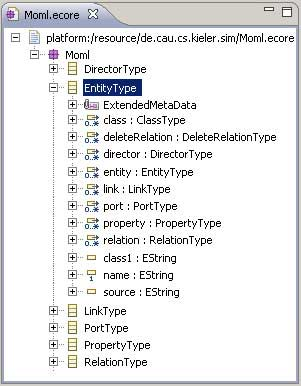
\includegraphics[scale=0.45]{images/MomlEcoreSimplified.jpg}
				}
   			\parbox{0.58\textwidth}{   
				\begin{itemize}
					\item Ptolemy models can be executable
					\pause
					\item DTD of the Ptolemy \\XML representation \emph{(MOML)}
					\pause
						\begin{itemize}
						\item Acquire EMF model
						\pause
						\item M2M transformation
						\pause
						\item Execute Ptolemy models
						\pause
						\item Back mapping of data/states
						\end{itemize}
					\end{itemize}
				}
		\end{tabular}	

  \end{frame}
%\note{} 


\subsection[Simulation Engine]{Simulation Engine}
%%%%%%%%%%%%%%%%%%%% Folie 11 %%%%%%%%%%%%%%%%%%%%%%%%
\begin{frame}
  \frametitle{Simulation with Ptolemy}
 % 		\only<1>{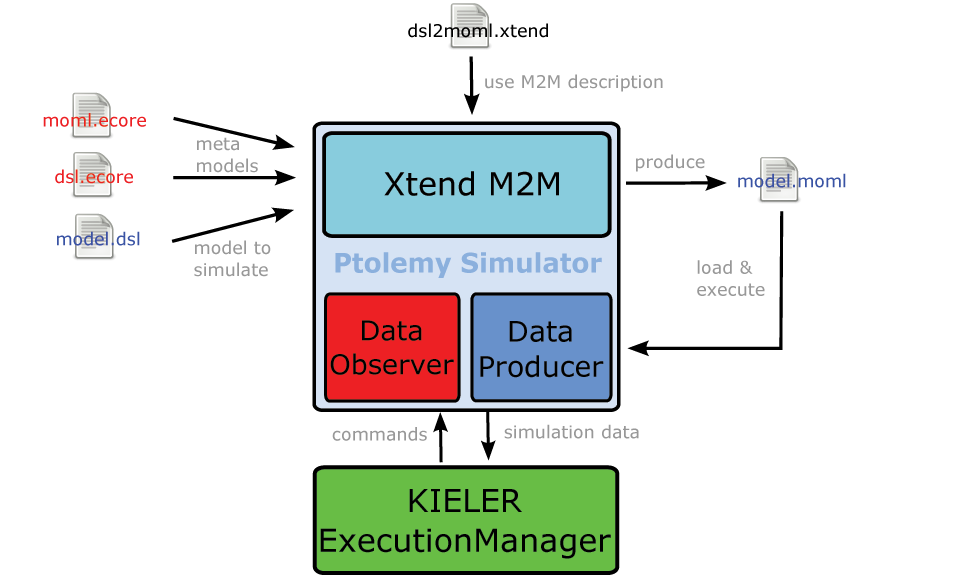
\includegraphics[scale=0.32]{images/KlePtoOverview.png} }
  		\only<2>{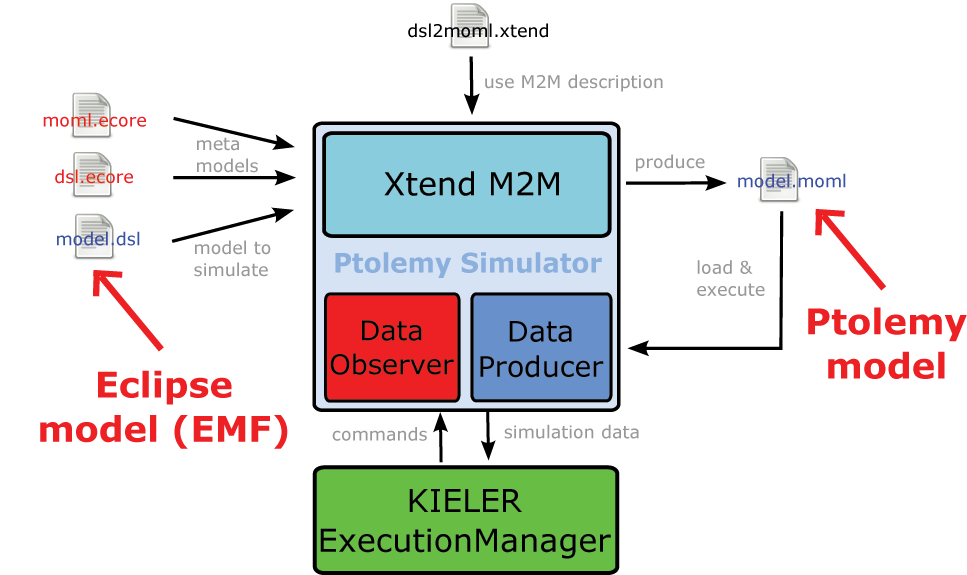
\includegraphics[scale=0.32]{images/KlePtoOverview2.png} }
  \end{frame}
%\note{} 



\section*{Use Case: Model Railway}
%%%%%%%%%%%%%%%%%%%% Folie 12 %%%%%%%%%%%%%%%%%%%%%%%%
\begin{frame}
  \frametitle{Overview}
    \begin{itemize}
	      \item \GRAY{KIELER Execution Manager}
	      \item \GRAY{Use case: Ptolemy }
        \begin{itemize}
       	       \item \GRAY{M2M transformation}
       	       \item \GRAY{Simulation engine}
        \end{itemize}
	      \item Use case: Model Railway
        \begin{itemize}
	            \item Installation
	            \item Railway Controller DSL
	            \item SimpleRailCtrl editor \emph{(DEMO)}
        \end{itemize}
	      \item \GRAY{Summary}
    \end{itemize}
\end{frame}
%\note{} 


\subsection<presentation>[Installation]{Installation}
%%%%%%%%%%%%%%%%%%%% Folie 13 %%%%%%%%%%%%%%%%%%%%%%%%
\begin{frame}
  \frametitle{Installation}
      \begin{figure}[t]
         \centering
         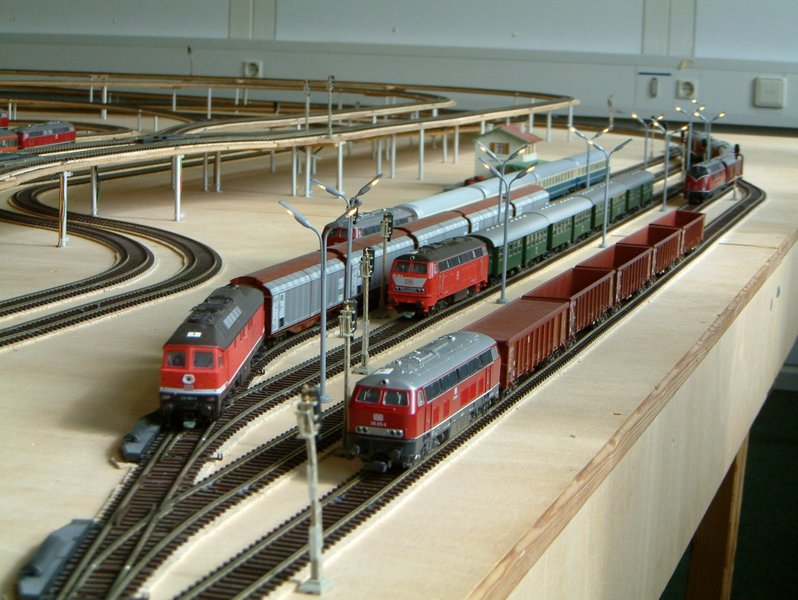
\includegraphics[scale=0.22]{images/railwayinstallation.jpg} 
       \end{figure}
\begin{itemize}
  \item Standard model railway equipment \pause combined with
  \pause
	\item Over 200 sensors and actuators
	\pause
	\item Controlled by distributed computer system
\end{itemize}
  \end{frame}
%\note{} 



%%%%%%%%%%%%%%%%%%%% Folie 14 %%%%%%%%%%%%%%%%%%%%%%%%
\begin{frame}
  \frametitle{Track Layout}
  \hspace{0.8cm}~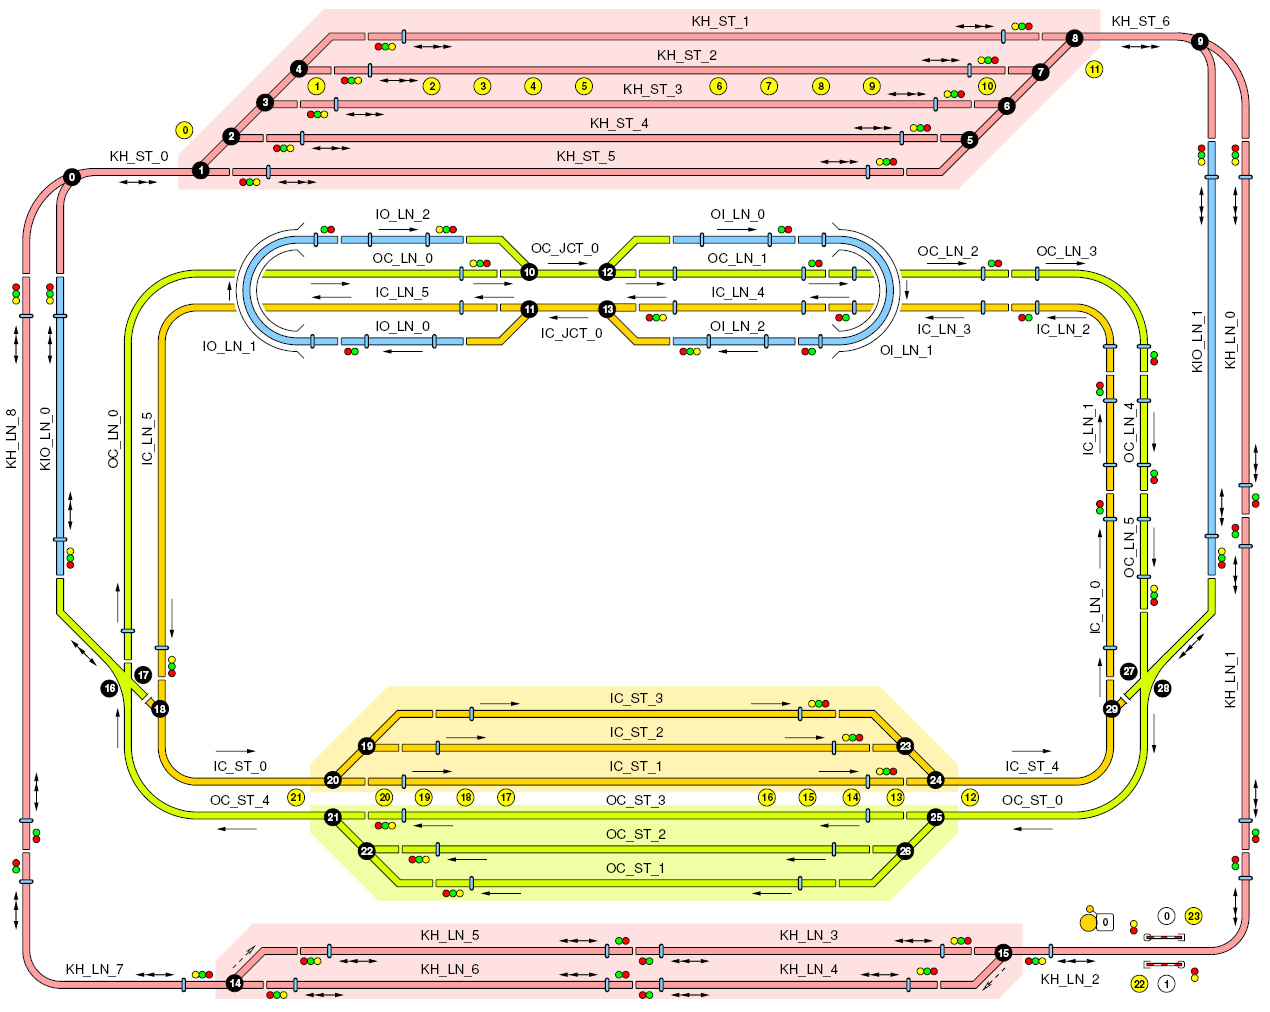
\includegraphics[scale=0.20]{images/tracksystem.jpg}
  \end{frame}
%\note{} 

\BackgroundPicture{images/nokiembackground.jpg}

%%%%%%%%%%%%%%%%%%%% Folie 15 %%%%%%%%%%%%%%%%%%%%%%%%
\begin{frame}
  \frametitle{Train Movement}
\hspace{1.5cm}~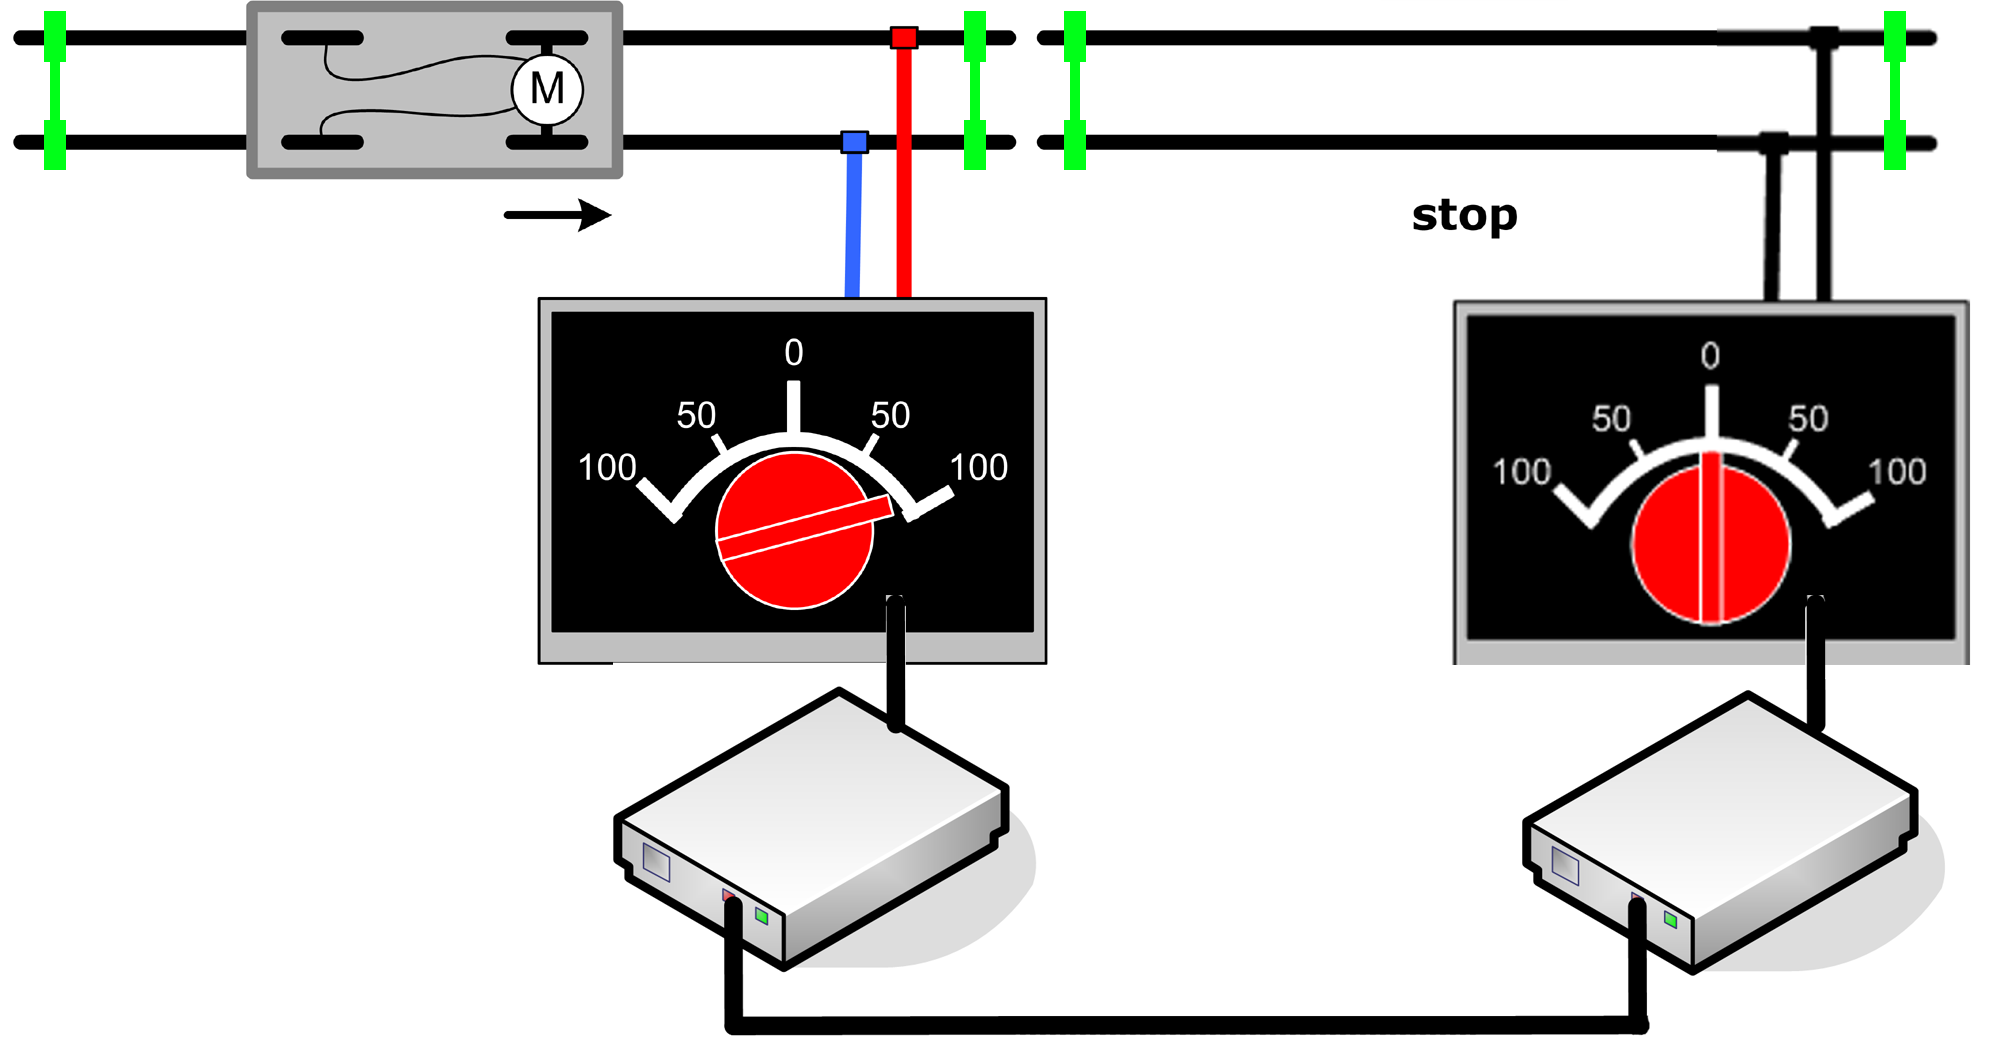
\includegraphics[scale=0.09]{images/segment-trains3.png}
\begin{itemize}
  \item Several track segments individually controlled 
  \pause
  \item Computers get sensor information (instantaneous train positions) and control voltage
  \pause
	\begin{itemize}
		  \item $\Rightarrow$ Actions: 
\includegraphics[scale=0.8]{images/SetSpeed.png} SetSpeed, 
\includegraphics[scale=0.8]{images/SetPoint.png} SetPoint
		  \item $\Rightarrow$ Trigger: 
\includegraphics[scale=0.8]{images/EventContact.png} EventContact, 
\includegraphics[scale=0.8]{images/EventWait.png} EventTimeout
	\end{itemize}
\end{itemize}
  \end{frame}
%\note{} 

\BackgroundPicture{images/kiembackground1.png}

\subsection<presentation>[Railway Controller DSL]{Railway Controller DSL}
%%%%%%%%%%%%%%%%%%%% Folie 16 %%%%%%%%%%%%%%%%%%%%%%%%
\begin{frame}
  \frametitle{EMF Meta Model}
\only<1>{\begin{figure}[t] \centering 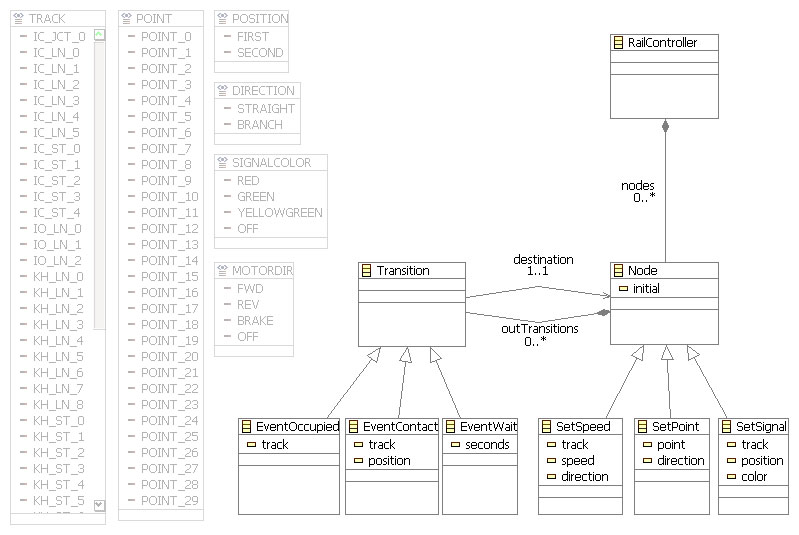
\includegraphics[scale=0.37]{images/SimpleRailCtrlMetaModel2.jpg}  \end{figure}}
	
\end{frame}
%\note{} 



\subsection<presentation>[SimpleRailCtrl Editor]{SimpleRailCtrl Editor}
%%%%%%%%%%%%%%%%%%%% Folie 17 %%%%%%%%%%%%%%%%%%%%%%%%
\begin{frame}
  \frametitle{Generated GMF Editor}
\begin{figure}[t] \centering 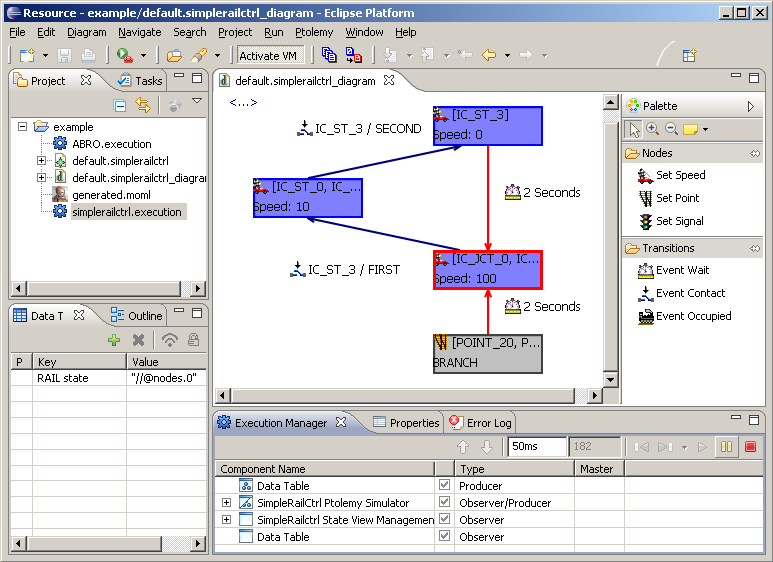
\includegraphics[scale=0.35]{images/simplerailctrleditor.png}  \end{figure}
	
\end{frame}
%\note{} 

%%%%%%%%%%%%%%%%%%%% Folie 18 %%%%%%%%%%%%%%%%%%%%%%%%
\begin{frame}
  \frametitle{Eclipse Model Execution Demo}
  \begin{center} 
      \textbf{\Large {LIVE DEMO}}
  \end{center}
  \end{frame}
%\note{} 

%invisible section
\section*{}

\subsection<presentation>[Summary]{Summary}
%%%%%%%%%%%%%%%%%%%% Folie 19 %%%%%%%%%%%%%%%%%%%%%%%%
\begin{frame}
  \frametitle{Summary}
        \begin{itemize}
	           \item DSLs in Eclipse represented by EMF models
								\begin{itemize}
									 \pause
				           \item Often only implicit execution semantics!
								\end{itemize}
						 \pause
	           \item Ptolemy models can be executable
								\begin{itemize}
				           \pause
	    			       \item Xtend M2M transformation helps making semantics explicit
								\end{itemize}
						 \pause
						 \item Other simulator DataComponents imaginable
						 \pause
						 \item \RED{KIELER Execution Manager} seamlessly integrates execution into the Eclipse RCP
        \end{itemize}
\end{frame}
%\note{}

\subsection<presentation>[To Go Further]{To Go Further}
%%%%%%%%%%%%%%%%%%%% Folie 20 %%%%%%%%%%%%%%%%%%%%%%%%
\begin{frame}
  \frametitle<presentation>[To Go Further]{To Go Further}
  \normalsize
  \bibliography{kiem-cmot}
  \invisible{
    \tiny
    \cite{www:kieler}
    \cite{www:ptolemy}
  }
\end{frame}
%\note{}

%\subsection<presentation>[The End]{The End}
%%%%%%%%%%%%%%%%%%%% Folie 21 %%%%%%%%%%%%%%%%%%%%%%%%
%\begin{frame}
%  \frametitle<presentation>[Thank you!]{}
%  \begin{center} 
%      \textbf{\Large Thank you for your attention and participation!}
%\\$ $\\
%      \textbf{\normalsize \BLUE{Any questions or suggestions?}} \\
%\invisible{
%\tiny
%\cite{www:kieler}
%\cite{www:ptolemy}
%}       
%      
%  \end{center}
%\end{frame}
%\note{} 

%%%%%%%%%%%%%%%%%%%%%%%%%%%%%%%%%%%%%%%%%%%%%%%%%%%%%%%%%%%%%%%%%%%%%%%%%%%%%%%
%\end{document}

